\subsection{Testing testing...}
This is where the testing results go

some numbers for now: Transfers running since March, some 2.6 million transfers, 86.8 percent success
rate, over 2 PB of data so far. Approx. 7 percent of the rate CMS achieves globally.

The mesh...

% To create this graphic:
% 1) save your image as a 1024x1024 png/gif/bmp
% 2) convert to pdf (install ImageMagick, then 'convert FileIn.png FileOut.pdf')
% N.B. if the input and output files have the same base name, LaTeX will prefer to take the png over the pdf,
% which is probably not what you want. Make sure the files have different names!
\begin{figure}[htp]
\centering
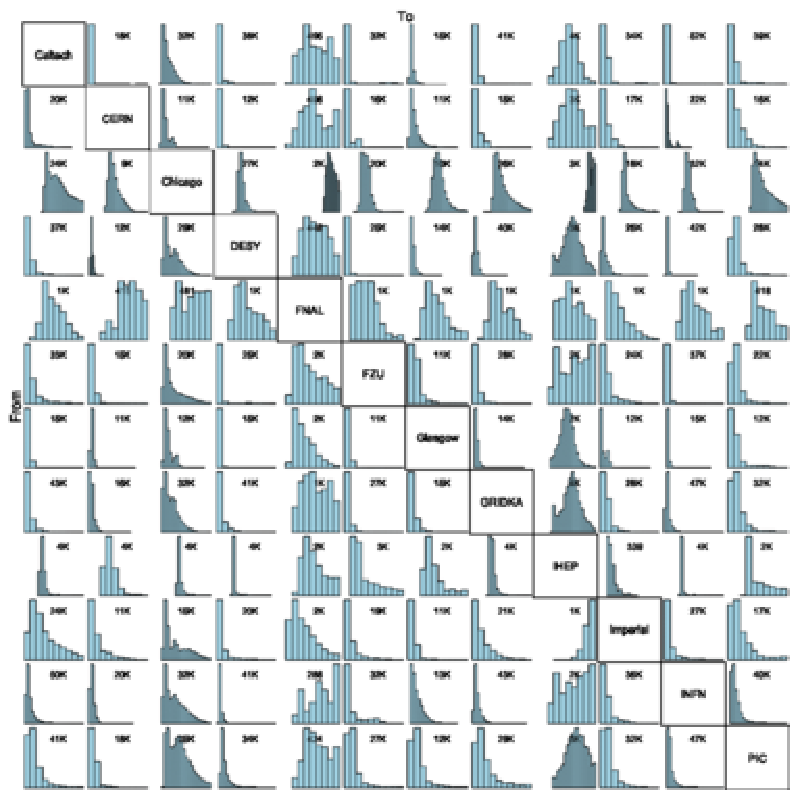
\includegraphics{full-mesh}
\caption{Transfer performance for the IPv6 testbed continuous transfers. A 1 GB file is transferred between each pair of sites, then deleted, then transferred again, continuously. The plots show the distribution of transfer duration times per site pair. The source site is named in the row, the destination site is named in the column. So the top-right plot shows transfers from Caltech to PIC, the bottom-left shows transfers fromPIC to Caltech. The x-axis is in seconds, from 0 to 500 for each plot. The number inset in each plot shows the approximate number of transfers between that site pair in that direction.}\label{fig:full-mesh}
\end{figure}

\begin{figure}[htp]
\centering
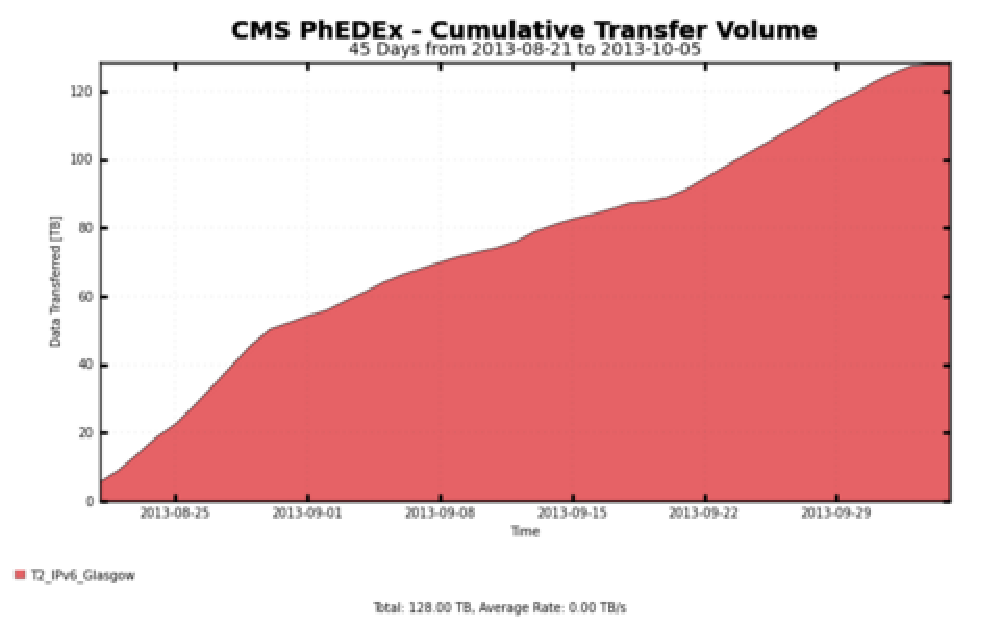
\includegraphics{phedex-transfer-volume}
\caption{Cumulative data-transfer between Imperial College and Glasgow using PhEDEx on the IPv6 testbed.}\label{fig:phedex-transfer-volume}
\end{figure}

